\chapter{Dataset}\label{chap:dataset}
In questo capitolo tratteremo la generazione del dataset posto alla base del modello che andremo a creare poi nel \autoref{chap:modello}. 
Vederemo prima il dataset originale utilizzato e poi come è stato aumentato tramite l'utilizzo di ulteriori analizzatori statici per migliorarne la precisione delle rilevazioni, andando a ridurre il numero di falsi positivi.
Verrà poi presentato come le rilevazioni degli analizzatori statici sono utilizzate per la associazione fra un \textit{code snippet} e il relativo errore, poi come da quest'ultimo venga ricavato il codice in formato di \textit{ast context vector}.

\section{Dataset originale}
Come detto in precedenza questo dataset non è stato generato partendo da zero, ma facendo riferimento al dataset creato da \cite{gelman2019source}. Il dataset consiste di circa 3000 progetti di GitHub, scritti in linguaggi C e \CPP,
 che rispettano due requisiti: hanno una licenza ridistribuibile e hanno almeno 10 stelle.
 Il secondo requisito ci serve per garantire che i progetti all'interno del dataset soddisfino dei requisiti di qualità, infatti come precedenti studi hanno mostrato (come ad esempio \cite{papamichail2016user}) si può utilizzare il numero
 di stelle su GitHub come un \textit{proxy} per la qualità del codice stesso.

Il dataset contiene per ogni progetto una serie di analisi effettuate: l'analisi di Doxygen che estrae le coppie codice-commento e l'analisi di Infer (scrivere che cosa è infer, magari con un footnote) che produce un report di analisi statica degli errori.
Visto l'utilizzo che ne sarebbe stato fatto di questo dataset, l'analisi di Doxygen è stata scartata. In \autoref{fig:dir_struct} si può vedere la struttura tipica di uno dei circa 3000 progetti presenti.
\begin{figure}
    \centering
    \scalebox{0.6}{
        \begin{forest}
            for tree={
                font=\ttfamily,
                grow'=0,
                child anchor=west,
                parent anchor=south,
                anchor=west,
                calign=first,
                inner xsep=7pt,
                edge path={
                  \noexpand\path [draw, \forestoption{edge}]
                  (!u.south west) +(7.5pt,0) |- (.child anchor) pic {folder} \forestoption{edge label};
                },
                % style for your file node 
                file/.style={edge path={\noexpand\path [draw, \forestoption{edge}]
                  (!u.south west) +(7.5pt,0) |- (.child anchor) \forestoption{edge label};},
                  inner xsep=2pt,font=\small\ttfamily
                             },
                before typesetting nodes={
                  if n=1
                    {insert before={[,phantom]}}
                    {}
                },
                fit=band,
                before computing xy={l=15pt},
              }  
        [Project-name
          [source
            [Project-name
                [Makefile, file]
                [File1.c, file]
                [File2.c, file]
                [..., file]
                [Folder1]
                [Folder2]
                [...]
            ]
          ]
          [derivatives
            [
                Infer-out
                [bugs.txt, file]
            ]
            ]
            [LICENSE, file]
            [url, file]
        ]
        \end{forest}
    }
    %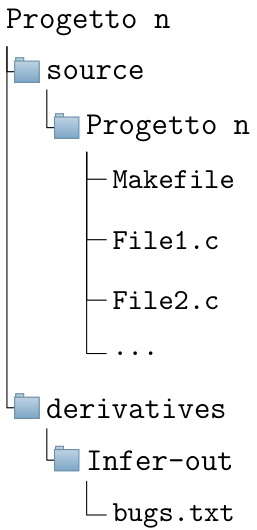
\includegraphics[scale=0.3]{images/immagineStrutturaDirectoryIniziale.png}
    \caption{La struttura della directory di un progetto del dataset iniziale}
    \label{fig:dir_struct}
\end{figure}

Come si può notare ogni progetto contiene anche un Makefile, elemento fondamentale perché gli analizzatori statici che andremo ad aggiungere spesso richiedono l'esistenza di un Makefile funzionante.

%Figura della struttura delle directory


%\subsection{Dataset originale}
 

%\subsection{Analizzatori utilizzati}

\section{Analizzatori di codice statici}
Un'analizzatore di codice è un programma che prende in input uno o più file e genera un report degli errori, cioè una lista di coppie del tipo $<$Errore, Posizione$>$, spesso in forma di file testuale. Di questi analizzatori ne esistono due macro categorie: statici e dinamici. 
Gli analizzatori statici sono programmi che effettuano controlli solo sul codice a livello testuale e che quindi non eseguono in nessuna maniera il codice. Gli analizzatori dinamici sono invece analizzatori più complessi che effettuano controlli a \textit{run-time}
andando quindi ad'eseguire il codice stesso.

Gli analizzatori non sono però perfetti, infatti nell'insieme degli errori trovati si possono spesso trovare dei falsi positivi, cioè frammenti di codice segnalati come erronei ma che in realtà non presentato nessun tipo di problema. Scopo appunto del dataset aumentato
è quello di ridurre il numero di falsi positivi.


\subsection{Analisi a livello di progetto} \label{subsec:compile_database}
La maggior parte degli analizzatori statici inoltre è in grado di lavorare a livello di progetti, andando quindi a risolvere correttamente gli \textit{include} (nel caso di C e \CPP), e quindi generando un output più significativo. 
Alcuni di questi per far ciò hanno bisogno di un file che viene chiamato \textit{compilation database} che mantiene informazioni sulla compilazione dei file del progetto. 
Per soddisfare questo requisito esistono strumenti appositi che utilizzano il Makefile per generarlo, nel caso di questo lavoro è stato utilizzato un programma chiamato Bear.


\subsection{Analizzatori utilizzati}
Come analizzatori sono stati utilizzati i seguenti quattro:
%Come analizzatori statici ulteriori da aggiungere in più a Infer, di cui ogni elemento del dataset ha già l'analisi sua associata, sono stati scelti i seguenti tre:
    \begin{itemize}
        \item L'analizzatore Cppcheck che ha tra i suoi punti di forza il minimizzare il numero di falsi positivi.
        \item GCC che, oltre ad'essere un compilatore, ha anche funzionalità per l'analisi statica dei programmi attraverso il parametro \textit{-fanalyzer}.
        \item Il compilatore Clang che attraverso un suo tool chiamato Clang-Check è in grado di effettuare analisi statiche.
        \item L'analizzatore Infer di cui il dataset è già dotato delle analisi per ogni progetto.
    \end{itemize}
Non sono stati usati analizzatori dinamici, questo perché il loro utilizzo in modo automatizzato è un operazione complicata se non quasi impossibile. 
Infatti quasi tutti i programmi prendono o dei parametri all'esecuzione o degli input durante l'esecuzione, ma fornire questi dati in modo consistente e sensato per il programma e in modo automatizzato rende il tutto veramente difficile.

L'utilizzo di essi però potrebbe portare a risultati molto interessanti poiché parte dei falsi positivi degli analizzatori statici deriva dal non poter decidere se frammenti di programmi sono o non sono eseguiti e quindi gli analizzano tutti.
Può infatti succedere che se in un frammento di programma che non viene sicuramente mai eseguito c'è un errore, l'analizzatore statico lo riferisce mentre quello dinamico, correttamente, no.


\section{Utilizzo efficace di processori multicore}
L'ultimo argomento da discutere prima di illustrare i passaggi della generazione del dataset è il tempo di esecuzione. 
Vista la mole di progetti e le loro dimensioni non irrilevanti se eseguissimo in modo \textit{naive} la generazione del dataset avremmo tempi di analisi che possono estendersi anche a periodi di giorni.
Dal momento che il processore utilizzato per la generazione del dataset è un processore multicore è stato deciso di ridurre i tempi di esecuzione delle fasi della generazione sfruttando ciò.
Python attraverso la sua libreria \textit{multiprocessing} permette infatti di eseguire la computazione in processi diversi, andando a ridurre drasticamente il tempo delle operazioni.
Quindi tutte le operazioni di seguito descritte, anche non facendone più menzione, saranno eseguite in questa maniera.

\section{Prima fase: generazione dei report degli errori}
La prima fase della generazione del dataset consiste quindi nell'utilizzare i tre analizzatori scelti per generare ulteriori report degli errori, in particolare:
    \begin{itemize}
      \item Per eseguire l'analizzatore di GCC vengono prima raccolti tutti i file sorgenti del progetto, cioè tutti quei file che terminano con ".c", ".cpp" o ".h". Una volta fatto ciò viene eseguito il seguente comando:
            \command{gcc -fanalyzer -Wall \args{files} 2\textgreater  gcc-bugs.txt}

            Il prodotto di questo comando sarà un unico file contente tutti gli errori e la loro posizione indicata con il percorso relativo del file e il numero sia della riga sia della colonna.
      \item Clang-check invece può essere eseguito su una cartella e quindi si occupa lui di trovare i file da analizzare.
             Non viene però utilizzato in questa modalità perché nel file di output finale al posto del percorso relativo dei file viene utilizzato solo il nome di questo, ma può succedere che in progetti grandi si abbiano file chiamati uguali ma in cartelle diverse.
             Per risolvere questo problema viene eseguito individualmente su ogni file tramite il comando:
              \command{clang-check -{}-analyze -p compile\_commands.json \args{file}}
            Come si può notare utilizza un file chiamato compile commands.json che è il file che è richiesto da certi analizzatori statici, come già detto nella \autoref{subsec:compile_database}.
            Gli output generati dall'esecuzione di questi comandi vengono poi processati andando a sostituire i nomi dei file con il loro percorsi relativi, e poi uniti tutti insieme. 
      \item Per finire viene poi eseguito cppcheck che invece non ha bisogno di nessun aggiustamento e si può eseguire direttamente su tutta la cartella contenente i sorgenti con il seguente comando:
            \command{cppcheck \args{cartella\_sorgenti} -{}-output-file=cppcheck-bugs.txt}
    \end{itemize}
    In \autoref{fig:grafo_errori_generati} possiamo vedere quanti errori sono stati generati da ogni singolo analizzatore.


    \begin{figure}
      \centering
      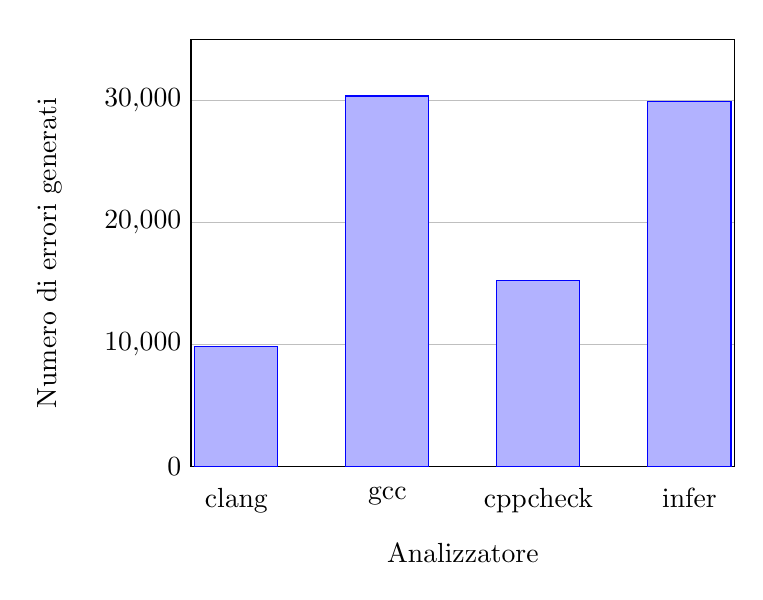
\begin{tikzpicture}
      \begin{axis}[
      width  = \textwidth * 0.7,
      height = 7cm,
      major x tick style = transparent,
      ybar=0.1pt,
      bar width=30pt,
      ymajorgrids = true,
      ylabel style={yshift=2ex},
      xlabel style={yshift=-1ex},
      xlabel=Analizzatore,
      ylabel=Numero di errori generati,
      symbolic x coords={clang,gcc,cppcheck, infer},
      xtick = data,
      scaled y ticks = false,
      ymin=0,ymax=35000,
      ytick style={draw=none},
      %extra y ticks = 100,
      %extra y tick labels={},
      %extra y tick style={grid=major,major grid style={very thick,draw=red}}
      ]
      \addplot table {
        Analizzatore Numero
        clang 9855
        gcc 30386
        cppcheck 15230
        infer 29950
      };
      \end{axis}
      \end{tikzpicture}
      \caption{Numero di errori generati da ogni analizzatore}
      \label{fig:grafo_errori_generati}
  \end{figure}


\section{Seconda fase: aggregazione dei report degli errori}
Dopo la prima fase descritta nella sezione precedente avremo come risultato quattro report di errori in file separati. Questi report si distinguono per due caratteristiche principali: la struttura del file e la nomenclatura degli errori. 
Per poter andare ad'utilizzare questi risultati, e fare quindi l'aggregazione di essi, dovremo effettuare due trasformazioni: un \textit{parsing} e una \textit{normalizzazione}.


\subsection{Parsing dei report}
Il \textit{parsing} è l'analisi di un dato in forma testuale per identificarne le sue componenti principali dove, in questo caso, sono la tipologia di errore e la sua posizione. 
Nel nostro caso è possibile eseguire il parsing tramite delle specifiche \textit{regex} che, avendo diversi formati di file, saranno diverse per ognuno degli analizzatori.
Il risultato del parsing sono quindi tanti record nella forma \record{errore, posizione}, dove la posizione indica sia il percorso del file ma sia anche la riga e la colonna dell'errore.

\subsection{Normalizzazione}
Per \textit{normalizzazione} si intende il processo di uniformare ad'un unico spazio di valori i dati forniti. Questo fase è fondamentale poiché i vari analizzatori forniscono lo stesso tipo di errore sotto nomi diversi. 
Per fare un esempio possiamo guardare la \autoref{tab:nomenclature} che riassume le diverse nomenclature per il tipo di errore 'memory leak'. 

\vskip1cm
    \noindent\setlength\tabcolsep{4pt}%
    \begin{tabularx}{\linewidth}{|l|c|*{4}{>{\RaggedRight\arraybackslash}X|}}
      \hline
      Forma normalizzata & Infer & Clang & Cppcheck & GCC \\ [0.5ex]
      \hline
      Memory leak  &  MEMORY\_LEAK  & unix.Malloc, ... & memleak, memleakOnRealloc, ... &  Wanalyzer-malloc-leak\\
      \hline
    \end{tabularx} 
    \captionof{table}{Tabella delle diverse nomenclature per l'errore 'memory leak'} \label{tab:nomenclature}
\vskip1cm

Notiamo inoltre un concetto fondamentale: analizzatori diversi producono analisi a granularità diverse. 
Si può osservare granularità maggiore, per il tipo di errore 'Memory leak', da parte di Cppcheck e Clang nella \autoref{tab:nomenclature}.
Infatti tutti e due definiscono più tipologie di errori che però, per convezione di questo progetto, vengono raggruppate in un'unica macro categoria.
Al contrario ci sono invece casi in cui un analizzatore non ha sensibilità sufficiente per distinguere fra due o più categorie di errori, in questa situazione un errore di quel tipo viene normalizzato in un errore per ogni categoria che potrebbe rappresentare, si può vedere ciò nella \autoref{tab:granularità}.
Nella eventualità quindi che Clang riferisca un errore di tipo 'unix.Malloc' dopo la fase di normalizzazione avremo due errori nella stessa posizione: uno di tipo 'Memory leak' e uno di tipo 'Use after free'. 

Per effettuare la normalizzazione è stata quindi sviluppata una tabella che associa ad'ogni forma normalizzata degli errori le forme definite dagli analizzatori usati.
Questa tabella è stata poi utilizzata come dizionario per convertire le tipologie di errori.

\begin{center}
  \begin{tabular}{|c|c|}
    \hline
    Forma normalizzata & Clang  \\
    \hline
    Memory leak  &  unix.Malloc, ... \\
    \hline
    Use after free & unix.Malloc, ... \\
    \hline
  \end{tabular}
  \captionof{table}{Tabella che mostra come un determinato errore di un analizzatore potrebbe corrispondere a più forme normalizzate} \label{tab:granularità}
\end{center} 

%vengono definiti più errori, nella stessa posizione, per ogni categoria che potrebbe rappresentare quell'errore.

\subsection{Aggregazione dei report}
Una volta definite le trasformazioni da effettuare possiamo introdurre l'effettivo argomento di questa sezione, cioè l'aggregazione dei quattro file prodotti dagli analizzatori.
Il processo di aggregazione permette di generare un unico report finale degli errori, andando a selezionare soltanto gli errori che sono stati individuati da almeno $n$ analizzatori. 
Modificando il parametro $n$ andremo, di conseguenza, a modificare la precisione e la dimensione del dataset nel seguente modo:
  \begin{itemize}
    \item Ponendo $n=1$ avremo la dimensione massima del dataset, in cui ogni singolo errore riportato viene mantenuto, a scapito però di un numero di falsi positivi più grande.
          Notiamo comunque, e questo vale per tutti i valori di $n$, che nel caso di errori duplicati ne viene sempre inserito solo uno.
    \item Ponendo $n=2$ avremo un bilanciamento fra precisione e dimensione del dataset. Vengono infatti selezionati tutti gli errori riferiti da almeno due analizzatori. 
        %Infatti come è stato notato empiricamente è alquanto raro che più di due degli analizzatori individuino un specifico errore,
          %quindi con $n=2$ manterremo comunque un sufficiente numero di dati migliorandone però la precisione.
    \item Ponendo $n>2$ invece il numero di errori selezionato diventa così basso che renderebbe difficile addestrare una rete, il numero però di falsi positivi diminuisce di conseguenza.
  \end{itemize}
Si può vedere in modo più chiaro come al variare del valore di $n$ cambi il numero di errori ottenuti in \autoref{fig:grafo_aggregazione}.
Nel caso di questo lavoro sono stati utilizzati dataset sia derivanti dal porre $n=1$ sia dal porre $n=2$.

\begin{figure}[h]
    \centering
    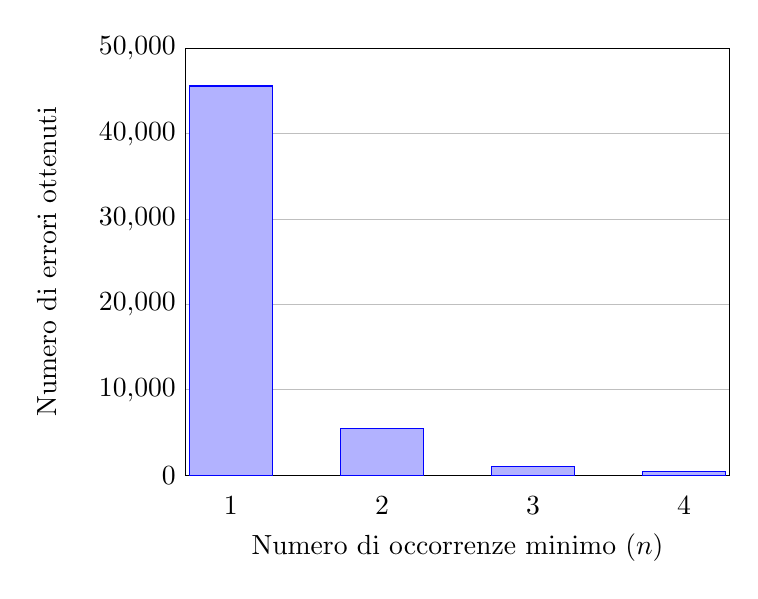
\begin{tikzpicture}
    \begin{axis}[
    width  = \textwidth * 0.7,
    height = 7cm,
    major x tick style = transparent,
    ybar=0.1pt,
    bar width=30pt,
    ymajorgrids = true,
    ylabel style={yshift=2ex},
    xlabel=Numero di occorrenze minimo ($n$),
    ylabel=Numero di errori ottenuti,
    xtick = data,
    scaled y ticks = false,
    ymin=0,ymax=50000,
    ytick style={draw=none},
    %extra y ticks = 100,
    %extra y tick labels={},
    %extra y tick style={grid=major,major grid style={very thick,draw=red}}
    ]
    \addplot table {
      N Numero 
      1 45606
      2 5423
      3 1049
      4 433
    };
    \end{axis}
    \end{tikzpicture}
    \caption{Numero di errori aggregati ottenuti in variazione del numero $n$ di occorrenze minime}
    \label{fig:grafo_aggregazione}
\end{figure}

\section{Terza fase: associazione tra errore e codice}
Lo scopo di questa fase è quello di mappare la posizione di ogni singolo errore ad'un determinato \textit{code snippet}. 
Prima di far ciò va definito però a che livello eseguire le analisi e quindi le successive predizioni del modello.
Le possibili strade che si possono intraprendere sono:
  \begin{itemize}
    \item A livello di file. Facendo ciò, dato un errore il \textit{code snippet} che associamo è il codice sorgente del intero file. 
          Questo metodo ha due vantaggi principali: la semplicità e la quantità d'informazioni codificate. 
          Ha però anche una serie di svantaggi: per il modello potrebbe essere troppo dispersivo per file grandi e dal momento che un singolo file è probabile che contenga più errori il modello dovrebbe restituire sequenze di predizioni.
    \item A livello di funzione. In questo caso si associa all'errore il blocco della funzione che lo racchiude.
          Il beneficio di ciò è la riduzione drastica del frammento di codice associato ad'un errore, rendendo più chiare le relazioni tra i vari elementi del codice e il tipo di errore.
    \item A livello di riga, in cui ad'un dato errore associamo come code snippet solo la riga stessa. In questo caso la dispersione sarà minima ma allo stesso tempo lo sarà la quantità d'informazioni a disposizione.
  \end{itemize}

In \autoref{fig:trade_off} possiamo notare il \textit{trade-off} che avviene tra l'aumentare della dimensione del code snippet e la quantità d'informazioni da esso incapsulata. 

Nel lavoro svolto è stato scelto di eseguire le analisi a livello di funzione, andando però ad aumentare il quantitativo d'informazioni a disposizione aggiungendo un contesto della funzione (la cui definizione verrà data in seguito nella \autoref{subsec:context}). 
Facendo questa scelta inoltre è possibile approssimare il problema ipotizzando che in una data funzione ci sia massimo un solo errore, rendendo quindi l'architettura del modello finale più semplice.

\begin{figure}
  \centering
  \begin{tikzpicture}
    \begin{axis}[
        xlabel={Quantita di informazioni},
        ylabel={Dispersività},
        yticklabels={,,},
        xticklabels={,,},
        xmin=0,    xmax=1,
        ymin=0,    ymax=1.718,
        axis line style={->},
        legend pos=south east
    ]
        \addplot[color=blue,domain=0:2,smooth, samples=400]{exp(x)-1};
        \addplot +[mark=none, color=red, dashed] coordinates {(0.5,0) (0.5, 0.649)};
        \addplot +[mark=none, color=red, dashed] coordinates {(0,0.649) (0.5, 0.649)};
    \end{axis}
    %
  \end{tikzpicture}
  \caption{\textit{Trade-off} che avviene tra la dispersività e la quantità di informazioni. Selezionando tanto codice avremo tante informazioni ma anche la dispersività aumentata, mentre selezionandone poco avremo poca dispersività ma potremmo perdere informazioni chiave.
    Le due linee rosse indicano un punto di bilanciamento tra i due.
  }
  \label{fig:trade_off}
\end{figure}

Una volta determinato il livello a cui svolgere le analisi possiamo tornare al problema principale: estrarre il codice della funzione che racchiude l'errore. 
Nonostante questo possa sembrare un problema semplice di analisi testuale vedremo come, in realtà, non lo sia.
Questo vale ancora di più per linguaggi come C e \CPP{} che, tramite la loro sintassi molto libera, rendono il tutto più complicato.
Prima di discutere di ciò dobbiamo quindi introdurre un concetto fondamentale: gli alberi di sintassi astratta.


\subsection{Alberi di sintassi astratta}
Un albero di sintassi astratta, o in breve \textit{ast} (dall'inglese \textit{abstract syntax tree}), è una rappresentazione ad albero della struttura sintattica astratta di un testo, nel nostro caso del codice sorgente.
Queste strutture sono spesso generate da parser specifici e vengono utilizzati come rappresentazione intermedia del programma in un processo di compilazione.

Possiamo vedere un esempio di albero prendendo il frammento di codice nello \autoref{code:esempio} scritto in uno pseudo-linguaggio.
Un possibile albero di sintassi astratta per questo frammento di codice è quello indicato in \autoref{fig:ast_esempio}.
Come si può vedere l'ast rappresenta in modo efficace la struttura completa del codice, andando ad'individuare e distinguere elementi come:
  \begin{itemize}
    \item Il corpo, la \textit{signature} e il valore di ritorno della funzione. 
    \item La dichiarazione della variabile 'total' e il blocco del for.
    \item I componenti del costrutto for: il corpo, la condizione, l'inizializzazione e lo step della variabile di controllo.
  \end{itemize}

  \begin{code}[caption={Frammento di codice che calcola la somma dei valori in un vettore}, label={code:esempio}]
    void foo(int[] array){
      int totale = 0;
      for(int i = 0; i < array.length; i++){
        totale = totale + array[i]
      }
      return totale;
    }
  \end{code}

\begin{figure}[h]
  \centering
  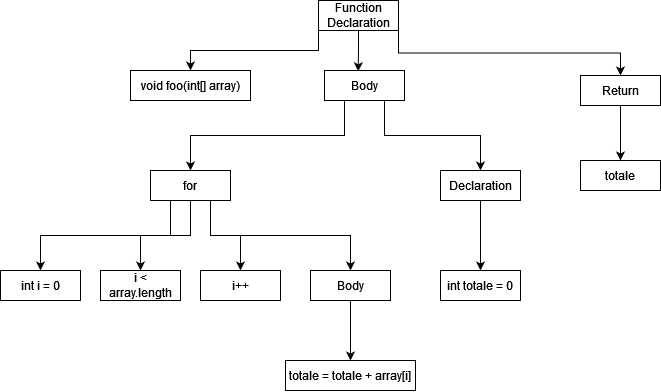
\includegraphics[scale=0.5]{images/astEsempio.png}
  \caption{Esempio di albero di sintassi astratta}
  \label{fig:ast_esempio}
\end{figure}

In questo progetto verranno utilizzati gli alberi di sintassi astratta per poter estrarre correttamente il codice della funzione che rinchiude l'errore. 
Questa operazione poteva anche essere fatta a livello testuale ricercando le parentesi graffe di apertura e chiusura della funzione. 
In questa maniera però sorgono casi problematici come l'utilizzo di parentesi graffe all'interno di commenti e/o stringhe che vanno ignorati o l'utilizzo particolare di direttive \textit{define}.
Tutto ciò rende il problema in apparenza semplice in realtà complesso.
A supporto di ciò vediamo lo \autoref{code:esempio_codice_complesso} in cui, nonostante sia codice \CPP{} completamente valido, l'individuazione del corpo della funzione che racchiude la linea di errore è un operazione tutt'altro che semplice.

\begin{code}[language=c++, caption={Esempio di codice valido con struttura particolare}, label={code:esempio_codice_complesso}]
  #DEFINE OPENBRACKET {
  #DEFINE CLOSEBRACKET }
  void foo()OPENBRACKET
    int error = 5 / 0; // Linea contente l'errore

    /* Questo commento rende difficile l'individuazione del corpo della funzione }
    */

  CLOSEBRACKET
\end{code}

\subsection{Generazione e parsing degli AST}
Come accennato nella precedente sezione in questo lavoro vengono utilizzati gli ast come metodo per estrarre i blocchi delle funzioni e il loro relativo contesto.
Prima di tutto bisogna essere in grado di generare un albero di sintassi astratta dato un file sorgente.
Per far ciò viene utilizzato il compilatore Clang che, attraverso flag specifiche, è in grado di generare un albero rappresentato in formato JSON.
Più in particolare per ogni file sorgente che vogliamo analizzare viene eseguito il seguente comando:
  \command{
    clang -Xclang -ast-dump=json \args{file}
  }
Il risultato di questa operazione è un file in formato JSON che rappresenta la struttura dell'albero. Prima però di proseguire questo file viene caricato e trasformato in una struttura ad albero vera e propria.

Oltre alla struttura sintattica del codice all'interno dei dizionari JSON sono presenti informazioni ulteriori come: indicazioni sulla riga degli elementi, sui tipi, sui riferimenti esterni e molto altro.
Tutte queste informazioni vengono poi usate sia per estrarre il codice ma sia per estrarre il contesto della funzione. 

\subsection{Contesto di una funzione} \label{subsec:context}
Definiamo in fine cosa si intende con contesto di una funzione.
Il contesto di una funzione è l'insieme di tutti quei riferimenti esterni che vengono effettuati all'interno del corpo della funzione stessa, possono includere quindi:
  \begin{itemize}
    \item Funzioni esterne.
    \item Variabili esterne.
    \item Definizioni di tipo esterne. Visto che le definizioni di tipo possono dipendere da altri tipi non primitivi, in questo caso, oltre al riferimento stesso vengono aggiunte anche le dipendenze di esso.
  \end{itemize}
L'idea posta alla base dell'includere questo contesto nel risultato finale è il poter dare al modello il maggior numero d'informazioni possibili mantenendo comunque limitata la dimensione dello snippet.
Senza di questo infatti, anche un umano, potrebbe non essere in grado di comprendere il codice o non poterne trarre conclusioni significative su di esso. 
Guardando infatti lo \autoref{code:esempio_codice_grafo_dipendenze}, senza l'inclusione nel risultato finale della variabile globale non potremmo determinare che nella funzione \textit{foo} ci sia effettivamente un errore di divisione per zero.

\begin{code}[language=c++, caption={Esempio di codice da cui ricavare dipendenze esterne }, label={code:esempio_codice_grafo_dipendenze}]

  typedef int typeA;
  typedef typeA typeB; 

  typedef float typeC;

  int variabileGlobale = 0;

  int bar(){
    ...
  }

  void foo(){
    typeB variable = 1; //riferimento di tipo esterno
    int var = 5 / variabileGlobale // errore
    
    result = bar();
    ...
  }

\end{code}

\subsubsection{Estrazione del contesto}\label{sec:estrazione_contesto}
Per l'estrazione del contesto vengono utilizzate le informazioni codificate nell'albero di sintassi astratta prodotto da Clang.
Solamente per le definizioni di tipo vengono anche incluse le relative dipendenze e per far ciò viene costruito un grafo delle dipendenze.

Il grafo delle dipendenze è un grafo diretto in cui un vertice $v$ rappresenta una dichiarazione di tipo mentre un arco $(u,v)$ rappresenta la dipendenza del tipo $u$ dal tipo $v$.
Prendiamo come esempio lo \autoref{code:esempio_codice_grafo_dipendenze}. 
Il contesto della funzione \textit{foo} in questo caso dovrà mantenere informazioni sulla definizione di \textit{typeB} che però dipende dalla definizione del \textit{typeA}.
Bisogna quindi costruire il grafo delle dipendenze dei tipi utilizzando le informazioni contenute all'interno dell'albero di sintassi astratta.
Possiamo vedere quindi il grafo delle dipendenze per questo specifico frammento di codice in \autoref{fig:grafo_dipendenze}.


\begin{figure}[h]
  \centering
  \begin{tikzpicture}
    \tikzset{vertex/.style = {shape=circle,draw,minimum size=1.5em}}
    \tikzset{edge/.style = {->,> = latex'}}
  
    % vertices
  \node[vertex] (typeB) at  (0,0) {typeB};
  \node[vertex] (typeA) at  (4,0) {typeA};
  \node[vertex] (int) at  (8,0) {int};
  \node[vertex] (typeC) at (2, -2) {typeC};
  \node[vertex] (float) at (6, -2) {float};
  %edges
  \draw[edge] (typeB) to (typeA);
  \draw[edge] (typeA) to (int);
  \draw[edge] (typeC) to (float);
  \end{tikzpicture}
  \caption{Grafo delle dipendenze di tipo per lo \autoref{code:esempio_codice_grafo_dipendenze}}
  \label{fig:grafo_dipendenze}
\end{figure}

Per poter ricavare quindi, una volta costruito il grafo delle dipendenze, le dipendenze delle dichiarazioni di tipo si può eseguire una visita in ampiezza partendo dal riferimento esterno stesso.
Nel caso della funzione \textit{foo} otterremo quindi, visto il riferimento esterno al tipo \textit{typeB}, due definizioni di tipo, quelle di \textit{typeB} e \textit{typeA}.  

\subsection{Esempio di risultato finale}
Riprendendo sempre lo \autoref{code:esempio_codice_grafo_dipendenze} avremo che il risultato finale dell'estrazione del metodo \textit{foo} è il seguente:


\begin{code}[language=c++, caption={Esempio di estrazione del codice della funzione foo insieme al contesto}, label={code:esempio_finale}]

  typedef int typeA;
  typedef typeA typeB; 
  int variabileGlobale = 0;
  int bar();
  void foo(){
    typeB variable = 1; //riferimento di tipo esterno
    int var = 5 / variabileGlobale // errore
    ...
  }

\end{code}

Notiamo quindi che la definizione del tipo \textit{typeC} non è inclusa poiché non utilizzata all'interno del corpo della funzione, mentre sia la variabile globale sia le due definizioni di tipo e sia la signature della funzione \textit{bar} sono incluse nel contesto.


\section{Quarta fase: Generazione degli AST-context}
Come accennato nell'introduzione teorica nel \autoref{chap:introduzione_teorica}, il modello che verrà utilizzato prenderà in input il codice sorgente processato sotto forma di \textit{ast context}, cioè delle triple della forma:
  \[\anglebra{x_s, p, x_t}\]

dove $x_s$ e $x_t$ sono rispettivamente il \textit{token start} e \textit{token end}, mentre $p$ è il \textit{path} come descritto in \cite{alon2019code2vec}.
A differenza però di come viene illustrato nell'articolo, in cui $x_s$ e $x_t$ sono un singolo valore, verranno utilizzati dei vettori di token di inizio e fine, nel tentativo di ridurre la dimensione dei vocabolari.
Per generare queste triple verrà utilizzato un tool chiamato \textit{astminer}.

\subsection{AstMiner}
Astminer rappresenta il lavoro descritto in \cite{kovalenko2019pathminer} ed è un tool che permette di estrarre gli ast context da file sorgenti scritti in vari linguaggi come Python, C/\CPP{} e Java.
Può essere utilizzato in due modi differenti:
  \begin{itemize}
    \item Come una libreria di Kotlin/Java.
    \item Come un tool standalone della CLI. Questo sarà il modo che verrà utilizzato nel progetto essendo stato scritto tutto in Python.
  \end{itemize}
Lo strumento è configurabile in svariati modi, l'uniche configurazioni rilevanti utilizzate sono:
  \begin{itemize}
    \item \'E stato utilizzato in modalità code2vec.
    \item Sono stati utilizzati i seguenti valori:
      \begin{itemize}
        \item maxPathContextsPerEntity $=200$
        \item maxPathLength $=20$
        \item nodesToNumbers $=$ false. Infatti i token sia del percorso sia di inizio e fine verranno gestiti non da astminer ma a livello dell'applicazione con vocabolari specifici.
      \end{itemize}
  \end{itemize}
Come però già accennato nell'introduzione di questa sezione, il prodotto di Astminer in realtà non è esattamente uguale a quello illustrato nel articolo di code2vec.
Infatti invece che avere dei singoli valori per $x_s$ e $x_t$, Astminer produce in output ast context che hanno token d'inizio e fine che sono vettori, scomponendo token complessi in token multipli.
\'E stato deciso di non modificare questa scelta poiché potrebbe portare alla riduzione notevole della dimensione del vocabolario dei token, andando a rendere più significativo ogni singolo token.

Questa fase è una delle fasi più lente di tutte, seconda solo all'esecuzione degli analizzatori statici.

\subsection{Generazioni vocabolari per i token e per i path}\label{subsec:vocab}
L'output dell'esecuzione di astminer, visto il parametro nodesToNumbers $=$ false, sono degli ast context dove ogni token è ancora in formato letterale.
Per essere utilizzabile questo formato deve però prima essere trasformato in un valore intero.
Tale valore intero rappresenterà l'indice del token letterale all'interno di uno specifico vocabolario.

Più in particolare vengono creati due dizionari diversi:
  \begin{itemize}
    \item Un dizionario dei token degli elementi dei cammini ($p$), che d'ora in avanti chiameremo \textit{path vocab}.
    \item Un dizionario dei token degli elementi terminali (i valori $x_s$ e $x_t$ del ast context). In questo caso lo chiameremo \textit{token vocab}.
  \end{itemize}
In \autoref{fig:grafo_vocab_size} possiamo vedere la dimensione dei due vocabolari.
Si può vedere come i due abbiano ordini di grandezza completamente differenti, questo può essere spiegato dal fatto che i token terminali racchiudono svariate tipologie di elementi come nomi di variabile e di metodi,
mentre i token dei cammini racchiudono solamente elementi sintattici fissi come possono essere costrutti come dichiarazioni, blocchi e operazioni.

  \begin{figure}
    \centering
    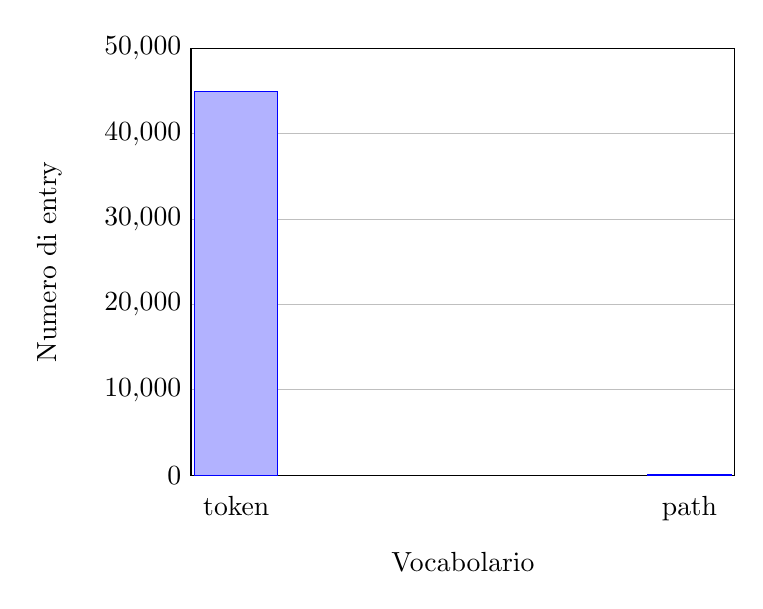
\begin{tikzpicture}
    \begin{axis}[
    width  = \textwidth * 0.7,
    height = 7cm,
    major x tick style = transparent,
    ybar=0.1pt,
    bar width=30pt,
    ymajorgrids = true,
    ylabel style={yshift=2ex},
    xlabel style={yshift=-1ex},
    xlabel=Vocabolario,
    ylabel=Numero di entry,
    symbolic x coords={token, path},
    xtick = data,
    scaled y ticks = false,
    ymin=0,ymax=50000,
    ytick style={draw=none},
    %extra y ticks = 100,
    %extra y tick labels={},
    %extra y tick style={grid=major,major grid style={very thick,draw=red}}
    ]
    \addplot table {
      vocab Numero
      token 45000
      path 50
    };

    \end{axis}
    \end{tikzpicture}
    \caption{Dimensione dei vocabolari dei token}
    \label{fig:grafo_vocab_size}
\end{figure}

  %TODO grafo dimensione vocabolari


%\subsection{Fase 1: utilizzo di analizzatori statici per la generazione di report di errori}

%\subsection{Fase 2: aggregazione dei report}

%\subsbusection{Conversione degli errori}

%\subsection{Fase 3: }

%\subsection{Fase 4: generazione degli Ast Context}

%\section{Statistiche finali del dataset}